\subsection{Управление памятью на основе регионов}
\subsubsection{Мотивировка}
Текущая реализация абстрактного синтаксического дерева имеет следующие 
недостатки:
\begin{enumerate}
    \item Выделение памяти стандартным методом может значительно фрагментировать
    оперативную память, затрудняя доступ к ней.
    \item Любое выделение и удаление памяти требует вмешательства системных
    вызовов, что может стать причиной дополнительных издержек во время
    работы программы.
    \item Программист не имеет возможности ручного управления выделяемой им
    памятью.
\end{enumerate}

Избавиться от этих недостатков можно используя различные оптимизации. В рамках 
этой работы воспользуемся управлением памятью на основе, так называемых, 
регионов (арен, зон) \cite{Wang}.

Под регионом далее будем понимать непрерывную область памяти, содержащую внутри 
себя объекты. При запуске программы выделим регион некоторого размера, при 
необходимости увеличивая его размер в некоторое постоянное
число раз.

Этот подход имеет следующие преимущества:
\begin{enumerate}
    \item Элементы располагаются последовательно, в связи с чем минимизируется
    фрагментация и упрощается доступ к объектам.
    \item Выделение и освобождение памяти выполняется с минимальными издержками
    \item Программисту предоставляется большая свобода для управления выделенной
    памятью.
\end{enumerate}

\subsubsection{Построение}
Формально определим требования к системе:
\begin{enumerate}
    \item Регион должен представлять из себя некоторый непрерывный участок 
    размера $n$ байт (в начальный момент времени размер равен некоторой 
    начальной величине $n_0$).
    \item При обращении к региону он должен предоставить $k$ байт памяти и 
    вернуть некоторый идентификатор этого участка для последующего обращения.
    \item При заполнении региона должна быть возможность увеличить объем 
    доступной памяти в некоторое число раз, которое далее будем называть
    коэффициентом увеличения.
    \item Должна быть доступна возможность эффективного освобождения всей 
    выделенной регионом памяти.
\end{enumerate}

Единственной сложной операцией над регионом является его увеличение.
Так как выделение нового участка потенциально может сопровождаться изменением 
адресов объектов, то необходимо организовать доступ к ним независимо от 
первоначального адреса. Для этого для каждого объекта будем получать доступ к 
нему через некоторый индекс. 

Кроме того, коэффициент увеличения должен быть выбран таким образом, чтобы был 
соблюден баланс между оптимальным объемом выделенной памяти и частотой системных
вызовов.

\subsubsection{Определение структуры}
Определим нашу структуру следующим образом:
\begin{minted}{cpp}
    typedef struct arena {
        // Указатель на начало региона
        struct node* arena;
        // Размер региона
        unsigned int size;
        // Объем выделенной регионом памяти
        unsigned int allocated;
    } arena;
\end{minted}

\subsubsection{Инициализация}
Теперь определим функцию \verb|arena_construct|, выполняющую начальную 
инициализацию состояния региона:
\begin{minted}{cpp}
    int arena_construct (arena* arena) {
        // Начальный размер региона равен некоторой постоянной, равной, DEFAULT_ARENA_SIZE
        arena->size = DEFAULT_ARENA_SIZE;
        arena->allocated = 0;
        // Выделим необходимое число памяти
        arena->arena = malloc(sizeof(node) * DEFAULT_ARENA_SIZE);
        // Если выделение прошло неудачно - вернем в качестве кода ошибки отличное, от 0 значение.
        if (arena->arena == NULL) {
            return (!0);
        }
    return 0;
    }
\end{minted}

\subsubsection{Выделение памяти}
После выделения некоторого объема памяти возможно обращение к ней.
Определим это обращение с помощью функции \verb|arena_allocate|:
\begin{minted}{cpp}
    int arena_allocate (arena* arena, unsigned int count) {
        // Если места в регионе недостаточно
        if (arena->allocated + count >= arena->size) {
            // Определим новый размер региона
            unsigned int newSize = MULTIPLY_FACTOR * arena->size;
            // Выделим регион большего размера и освободим ранее занятую память
            node* newArena = realloc(arena->arena,
            newSize * sizeof(node));
            if (NULL == newArena) {
                return -1;
            }
            arena->arena = newArena;
            arena->size = newSize;
        }
        // В качестве результата вернем индекс первого свободного участка региона
        unsigned int result = arena->allocated;
        // Сместим индекс на объем выделенной памяти
        arena->allocated += count;
        // Вернем результат
        return result;
    }
\end{minted}
Отметим, что наиболее часто значением \verb|MULTIPLY_FACTOR| оказывается числа
1.5 и 2. Это позволяет достичь амортизационно константного времени выполнения 
операции выделения памяти \cite{Fbdoc}.

\subsubsection{Освобождение выделенной памяти}
Наконец, реализуем освобождение выделенной региону памяти с помощью функции 
\verb|arena_free|
\begin{minted}{cpp}
    void arena_free (arena* arena) {
        if (arena->arena != NULL)
            free(arena->arena);
        arena->arena = NULL;
    }
\end{minted}

\subsubsection{Модификация абстрактного синтаксического дерева}
Осталось изменить исходный код программы, чтобы обеспечить выделение памяти с 
помощью полученной нами структуры данных.

Для этого воспользуемся директивой \texttt{\%param} и заявим в качестве 
параметра переменную типа \texttt{arena*}. В функциях \texttt{eval}, 
texttt{newnum}, \texttt{newast} внесем изменения, чтобы обеспечить выделение 
памятью с помощью написанных ранее функций.

С полным кодом программы можно ознакомиться в приложении \ref{app:A}.

\subsubsection{Сборка проекта}
Теперь проект можно собрать, незначительно изменив \texttt{Makefile}:
\begin{minted}{cpp}
    calc.out: calc.l calc.y arena_ast.h
        bison -d calc.y
        flex calc.l
        cc -o $@ calc.tab.c lex.yy.c arena_ast.c arena.c
\end{minted}
и запустить. Результат работы программы представлен на рис. \ref{img:demon}
\begin{figure}[H]
    \centering
    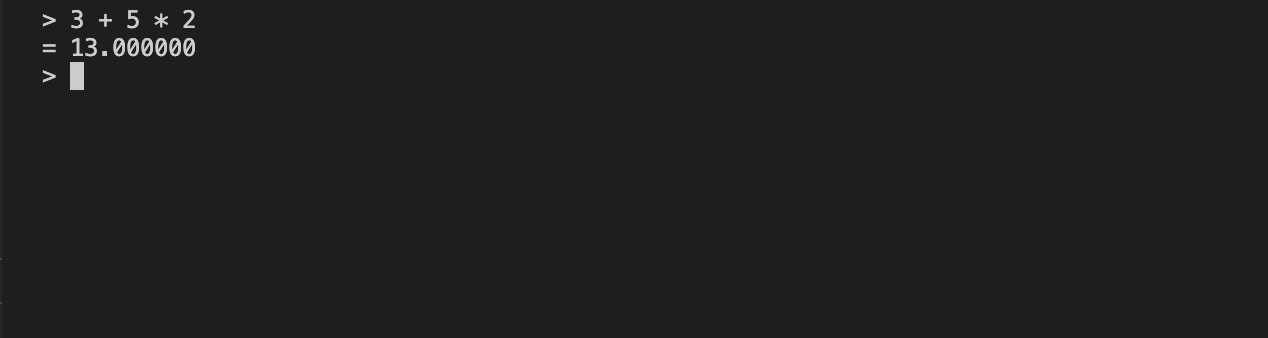
\includegraphics[width=0.65\textwidth]{naivetest.png}
    \caption{Демонстрация работы программы}
    \label{img:demon}
\end{figure}    
